\documentclass[11pt]{book}
\title{\textbf{Citogenetica e Ingegneria Cromosomica}}
\author{Simona Debilio}
\date{A.A. 2018/2019}
% manually added packages
\usepackage[margin=1in]{geometry}
\usepackage[italian]{babel}
% ====================================================
\usepackage{lmodern}
\usepackage{amssymb,amsmath}
\usepackage{ifxetex,ifluatex}
\usepackage{fixltx2e} % provides \textsubscript
\ifnum 0\ifxetex 1\fi\ifluatex 1\fi=0 % if pdftex
  \usepackage[T1]{fontenc}
  \usepackage[utf8]{inputenc}
\else % if luatex or xelatex
  \ifxetex
    \usepackage{mathspec}
    \usepackage{xltxtra,xunicode}
  \else
    \usepackage{fontspec}
  \fi
  \defaultfontfeatures{Mapping=tex-text,Scale=MatchLowercase}
  \newcommand{\euro}{€}
\fi
% use upquote if available, for straight quotes in verbatim environments
\IfFileExists{upquote.sty}{\usepackage{upquote}}{}
% use microtype if available
\IfFileExists{microtype.sty}{%
\usepackage{microtype}
\UseMicrotypeSet[protrusion]{basicmath} % disable protrusion for tt fonts
}{}
\ifxetex
  \usepackage[setpagesize=false, % page size defined by xetex
              unicode=false, % unicode breaks when used with xetex
              xetex]{hyperref}
\else
  \usepackage[unicode=true]{hyperref}
\fi
\hypersetup{breaklinks=true,
            bookmarks=true,
            pdfauthor={},
            pdftitle={},
            colorlinks=true,
            citecolor=blue,
            urlcolor=blue,
            linkcolor=magenta,
            pdfborder={0 0 0}}
\urlstyle{same}  % don't use monospace font for urls
\setlength{\parindent}{0pt}
\setlength{\parskip}{6pt plus 2pt minus 1pt}
\setlength{\emergencystretch}{3em}  % prevent overfull lines
\setcounter{secnumdepth}{0}

\date{}

\setlength{\parindent}{0pt}

\usepackage{graphicx}
\usepackage{caption}
\usepackage{subcaption}
\usepackage{siunitx}
\usepackage{wrapfig}

\begin{document}

\maketitle

\tableofcontents

\chapter{Programma}

Il programma delle lezioni prevede:

\begin{itemize}
\item 
Cenni storici;
\item 
Citogenetica classica e nuova;
\item 
Condensazione del DNA nel cromosoma eucariotico:

	\begin{enumerate}
	\item strutture ad anse e ruolo regolativo;
	\end{enumerate}

\item 
Metodi di localizzazione genica:

	\begin{enumerate}
	\item
	Ibridazione di cellule somatiche;
	\item 
	Ibridazione in situ;
	\end{enumerate}

\item 
Regolazione dell’espressione genica negli eucarioti multicellulari:

	\begin{enumerate}
	\item 
	Puffering (cromosomi politenici);
    \item 
    Trascrizione rDNA (cromosomi a spazzola);
    \item
    Determinazione del sesso;
    \item
    Compensazione del dosaggio nei mammiferi;
    \item
    Compensazione del dosaggio in Drosophila;
    \end{enumerate}

\item 
Imprinting genomico;
\item
Struttura del genoma degli eucarioti:

	\begin{enumerate}
    \item
    Progetti genoma;
    \item 
    Sequenze uniche e ripetute;
    \item
    Non coding RNA;
    \end{enumerate}
    
\item 
Citogenetica dei tumori:

	\begin{enumerate}
	\item
	Generalità;
    \item
    Esempi specifici: linfoma di Burkitt, LMC ph+, Retinoblastoma;
    \end{enumerate}
    
\item
Instabilità genomica:

	\begin{enumerate}
	\item
    Duplicazioni segmentali;
    \item
    Disordini genomici;
    \item
    Duplicazioni segmentali;
    \end{enumerate}
    
\item
Elementi funzionali del cromosoma eucariotico:

	\begin{enumerate}
    \item
    Telomeri;
    \item
    Origini di replicazione;
    \item
    Centromeri:
    \end{enumerate}
    	
		\begin{itemize}
        \item
        DNA centromerico;
        \item
        Proteine centromeriche;
        \item
        Paradosso del centromero;
        \item
        I centromeri nell’evoluzione;
        \end{itemize}
        
\item
Ricostruzione del cromosoma:
	
	\begin{enumerate}
    \item
    Cromosomi artificiali;
    \item
    Vettori cromosomici;
    \item
    Cromosomi artificiali di mammifero;
    \item
    Metodo bottom-up;
    \item
    Metodo bottom-down
    \end{enumerate}

\item
Terapia genica:

	\begin{enumerate}
    \item
    Terapia genica germinale;
    \item
    Terapia genica somatica;
    \item
    Terapia genica nei tumori;
    \item
    Problemi etici;
    \end{enumerate}

\item
Cellule staminali:

	\begin{enumerate}
    \item
    cellule staminali embrionali;
    \item
    cellule embrionali fetali e adulte;
    \item
    cellule iPS (inuced Pluripotent Stem Cells);
    \end{enumerate}
    
\item
Clonazione:

	\begin{enumerate}
    \item
    clonazione vegetale;
    \item
    conazione animale;
    \item
    clonazione terapeutica;
    \item
    clonazione riproduttiva;
    \item
    problemi etici.
    \end{enumerate}
\end{itemize}

\chapter{Introduzione}

La condensazione del DNA nel cromosoma eucariotico presenta un ruolo regolativo importante e rappresenta la base della regolazione epigenetica dell’espressione genica.

I cromosomi politenici di Drosophila sono, ad oggi, protagonisti della genetica molecolare. Drosophila continua infatti ad essere un ottimo modello per lo studio degli eucarioti poiché:
\begin{itemize}
\item
il numero di marcatori conosciuti è elevato;
\item
consente di seguire i diversi stadi di sviluppo;
\item
è un modello trasferibile negli eucarioti superiori.
\end{itemize} 

Un cromosoma politenico è un cromosoma gigante. I cromosomi politenici si formano in seguito a vari cicli di replicazione che producono molte copie (anche centinaia) di cromatidi fratelli che rimangono uniti.
La formazione dei cromosomi politenici ha la funzione di aumentare il volume cellulare ma può anche comportare un vantaggio metabolico dato che l'elevato numero di copie di geni permette un alto livello di espressione genica. In Drosophila melanogaster, per esempio, i cromosomi delle ghiandole salivari delle larve subiscono numerosi cicli di endoreplicazione, e questo consente di produrre grandi quantità di secreto prima dell'impupamento.
Al microscopio i cromosomi politenici mostrano caratteristici pattern di bande chiare e scure che possono essere utilizzati per identificare riarrangiamenti cromosomici e delezioni. Bande scure corrispondono spesso alla cromatina inattiva, mentre bande chiare si trovano di solito in aree con una maggiore attività trascrizionale.

La citogenetica è una branca della genetica. Il termine \emph{citogenetica} significa ``studio dei cromosomi'', si tratta quindi di una disciplina confinata alla descrizione dei cromosomi basata sull’utilizzo del microscopio.
In realtà oggi la citogenetica è descritta in maniera differente poiché, nel tempo, si è adeguata alle esigenze della biologia molecolare diventando strettamente complementare alle nuove tecnologie, note come post-genomica, che hanno raggiunto delle capacità descrittive, risolutive, e funzionali elevate; la citogenetica risulta quindi essere complementare alla genomica-post genomica. 

L’\emph{ingegneria cromosomica} rappresenta, invece, lo studio molecolare dei cromosomi utile per la costruzione di cromosomi artificiali.  

\section{Citogenetica classica e nuova citogenetica}
La citogenetica classica è una disciplina più vecchia della genetica, che nasce con la scoperta del microscopio e che su di esso si basa. Già i primi microscopisti, analizzando gli apici radicali delle piante e alcuni tessuti di organismi molto semplici, videro che vi erano delle cellule che subivano dei cicli di divisione cellulare e descrissero dettagliatamente i processi di meiosi e mitosi, prima ancora che nascesse la genetica.

La \textbf{citogenetica classica} consiste nello studio morfologico, al microscopio, del comportamento dei cromosomi alla mitosi e alla meiosi. 
Già i primi microscopisti si resero conto del fatto che vi fosse una grossa differenza tra ciò che avveniva nelle cellule mitotiche e in quelle meiotiche; essi infatti descrissero la segregazione dei cromosomi con una distribuzione equivalente del materiale genetico nelle cellule figlie durante la mitosi e scoprirono, invece, che vi erano alcuni tessuti in cui avveniva un dimezzamento del numero cromosomico a seguito della formazione dei gameti. Quanto scoperto a quei tempi risultò essere di difficile comprensione, ma risultò poi essere molto chiaro nel momento in cui la citogenetica e la genetica mendeliana si unirono in un’unica cosa che permise di capire che il comportamento dei cromosomi spiegava l’eredità mendeliana.

La citogenetica ha avuto una grossa spinta grazie all’evoluzione delle nuove tecnologie in campo umano, infatti già alla fine degli anni '50 questa disciplina risultò essere fondamentale per l’analisi del cariotipo umano normale e patologico, cioè per capire quali fossero le basi cromosomiche di alcune patologie e per la diagnosi delle stesse.

Fondamentali per poter identificare i cromosomi sono le tecniche di colorazione differenziale e le colture in vitro di cellule somatiche (i cromosomi risultano essere visibili durante la divisione cellulare). Se per i primi microscopisti lo studio dei tessuti meristematici degli apici radicali, trattandosi di tessuti in continua rigenerazione, non risultò essere difficile, lo studio dei cromosomi durante la divisione cellulare risultò invece più arduo a causa della difficoltà nel ritrovare tessuti in attiva rigenerazione spontanea nell’uomo. Tessuti di questo tipo ve ne sono, ma risultano essere difficilmente raggiungibili con tecniche non invasive (es. midollo osseo, tessuti tumorali e tessuti germinali).
Per questo motivo sono state sviluppate delle tecniche in grado di stimolare la proliferazione di tessuti differenziati che normalmente non si dividerebbero. Il tessuto di elezione è rappresentato dal sangue periferico, è infatti possibile indurre le cellule nucleate (linfociti) a proliferare; lo stesso può essere fatto effettuando dei piccoli espianti cutanei prelevando qualche mm\(^2\) di tessuto sottocutaneo.

La citogenetica classica è stata, fondamentalmente, la base delle leggi di Mendel. In passato vi fu un momento in cui la citogenetica classica, con l’avvento della biologia molecolare, sembrava fosse divenuta incapace di descrivere dettagli, soprattutto funzionali, che invece la biologia molecolare poteva arrivare a definire; veniva infatti considerata una ``cenerentola o un’ancella povera'' come quasi tutte le discipline morfologico-descrittive.
In realtà vi fu un’evoluzione sempre più veloce tale per cui la nuova citogenetica rappresenta sempre lo studio dei cromosomi ma con delle tecniche ad altissima risoluzione, fino ad arrivare a livelli di risoluzione comparabili a quelli della biologia molecolare delle analisi di sequenza.
La nuova citogenetica è quindi, a tutt’oggi, la base fisica della genetica, della biologia molecolare e della biologia strutturale perché permette di descrivere l’anatomia molecolare del cromosoma arrivando, addirittura, a ricostruirlo. 

Dal momento che la citogenetica possiede una visione d’insieme, risulterà essere molto importante perché rappresenterà il punto di partenza e di arrivo per l’analisi dei genomi complessi. Infatti, una volta stabiliti dei dettagli molecolari è importante poterli inserire in un contesto cromatinico definito, sarà proprio in questa fase che risulterà essere fondamentale la citogenetica.
Oggi è possibile fare una citogenetica di nuova generazione, basata sull’uso della citogenetica in assenza dei cromosomi e nota come citogenomica.

La patologia costituzionale e la citogenetica oncologica trovano un supporto insostituibile nello sviluppo di tecniche ad alta risoluzione che ad oggi permettono di fare delle descrizioni dettagliate delle diverse anomalie associate al cancro. Con la citogenetica è possibile stabilire, a livello molecolare, i punti di rottura coinvolti nei ri-arrangiamenti e, quindi, delimitare delle regioni critiche all’interno delle quali cercare oncogeni o oncosoppressori coinvolti nello sviluppo di quel particolare tipo di tumore; ciò risulterà avere un’importanza diagnostica e pronostica.

\section{Il cromosoma}
Il termina cromosoma è stato introdotto nel 1888 da Wilhelm Waldeier e classicamente risulta essere definito come \emph{un ``corpo colorato'' evidenziabile con coloranti basici durante la divisione cellulare} (mitosi, meiosi).

In realtà, ad oggi, la definizione appena data risulta essere superata poiché è definibile come cromosoma \emph{una qualsiasi molecola di acido nucleico che contenga l’informazione per la sintesi di tutte le proteine di un certo organismo, dotata di replicazione autonoma (origini di replicazione), circolare o lineare (nel secondo caso dotata di telomeri) e in grado di segregare fedelmente nelle cellule figlie (funzione espletata dal centromero).}

Il cromosoma eucariotico, durante la metafase, è costituito da due cromatidi fratelli (identici) legati al centromero. Ogni cromatidio è una molecola di DNA lineare e la ricombinazione tra cromatidi fratelli non determina un ri-arrangiamento cromosomico, ma solamente uno scambio di elementi.\\
In ogni eucariote diploide ogni cromosoma è presente in due copie, uno di origine materna e uno di origine paterna, tra loro omologhi. Gli omologhi non sono identici ma possono differire per varianti alleliche a tutti i loci.
Quanto appena detto risulterà essere particolarmente importante poiché rappresentante la base della replicazione sessuata e, quindi, la base della variabilità degli organismi.  

Il microscopio elettronico non aggiunge dettagli alla struttura del cromosoma poiché lo mostra semplicemente più grande e rappresentato da un caotico super-avvolgimento di una fibra non meglio identificata.\\
Il cromosoma eucariotico è formato da un braccio corto (\emph{p}, petit - la prima conferenza per la standardizzazione della nomenclatura citogenetica si svolse in Francia) e uno lungo (\emph{q} - ordine alfabetico).\\
Prendendo come riferimento il cariotipo umano, in ogni cromosoma la molecola è lunga \emph{da 45 a 285 milioni (10\(^6\)) pb}, contiene qualche migliaio di origini di replicazione, mediamente qualche migliaio di geni, un centromero e due telomeri.
Dopo la fase di sintesi del DNA ogni cromosoma è formato da due cromatidi fratelli che sono identici; ogni cromatidio è una doppia elica di DNA.

Il 1980 è la data di nascita delle tecnologie del DNA ricombinante che hanno dato l’avvio alla genetica e alla biologia molecolare. Nel 1981 Tomas Caskey, direttore del Baylor College of Medicine di Huston (USA), affermò su una famosa rivista scientifica che la citogenetica si sarebbe estinta entro 5 anni proprio perché di fronte alle enormi potenzialità delle nuove tecnologie sembrava che essa avesse esaurito le sue capacità descrittive, pur restando fondamentale per la parte diagnostica. 
Tuttavia, nel 1991, lo stesso Caskey, nella medesima rivista, affermò che la citogenetica avrebbe rappresentato l’onda del futuro. 

\subsection{Livelli di risoluzione}
\begin{itemize}
\item 
Un genoma umano aploide è costituito da 3 x 10\(^8\) pb (10\(^8\) = 100 milioni).
\item
Ogni cromosoma è costituito da 10\(^8\) bp.
\item
Una banda metafasica (unità visibile con colorazioni differenziali) presenta una dimensione di circa 10\(^7\) bp, mentre le dimensioni di una banda profasica saranno di 10\(^6\) pb; ci si avvicina sempre di più alle dimensioni del singolo gene.
Infatti lo sviluppo dei bandeggi ad alta risoluzione è stato un primo step utile a colmare quei vuoti presenti tra approcci citogenetici e molecolari.
\item
Le dimensioni di un gene risultano essere di 10\(^4\)-10\(^5\) bp.
\end{itemize}

L’esigenza di analizzare genomi sterminati, come quelli dei mammiferi, ha determinato lo sviluppo di tecniche molecolari che permettessero di fare analisi di segmenti genomici sempre più grandi.\\
Gli approcci classici permettevano di isolare e clonare segmenti di DNA nell’ordine del migliaio di pb, ma dovendo riempire di marcatori un genoma di 3 miliardi di pb, con soli pezzi di 1000 pb non si arriverà ad esprimere nulla. Sono quindi state sviluppate delle tecniche molecolari come il clonaggio in cromosomi artificiali batterici che permettono di isolare, maneggiare, sequenziare e descrivere segmenti che arrivano a 10\(^5\)-10\(^6\) bp, dimensioni delle bande che si analizzano con i bandeggi ad alta risoluzione.\\
La citogenetica molecolare di ultima generazione, in grado di estrarre il DNA e pettinarlo sui vetrini, permette di arrivare ad una risoluzione di alcune centinaia di pb. Le nuove tecnologie hanno quindi permesso di colmare quel vuoto tra approccio morfologico e molecolare. 
In realtà i due approcci sono complementari poiché quello molecolare è indiretto e necessita di un’interpretazione e di un’analisi statistica dei risultati, mentre il grosso vantaggio dell’approccio citogenetico è quello di poter confermare i risultati con un metodo visivo; sarà infatti possibile osservare al microscopio le sequenze di DNA e questo risulterà essere fondamentale perché è vero che la risoluzione è inferiore, ma si avrà una prova del fatto che le molecole che si era ipotizzato essere così organizzate lo saranno effettivamente e, trattandosi di un approccio fisico, sarà inoltre possibile orientare tali molecole, cosa che non sarà possibile fare interpretando la dimensione delle bande visibili su di un gel. 
Pertanto risoluzione e approcci differenti forniranno, insieme, un’informazione completa per capire la struttura di genomi complessi come quelli dei mammiferi.

\subsection{La teoria cromosomica dell’eredità}
La teoria cromosomica dell’eredità si basa sulla fusione delle informazioni ottenute dai primi microscopisti sul comportamento dei cromosomi alla meiosi e alla mitosi con le leggi di Mendel.\\
Nel 1887 Weismann, effettuando analisi microscopiche, descrisse il comportamento dei cromosomi affermando quanto segue:
\begin{itemize}
\item 
la sostanza nucleare alla mitosi si divide in maniera equivalente nelle cellule figlie;
\item
se si parla di cellule meiotiche, i gameti femminili perderanno metà della sostanza nucleare nel secondo globulo polare, che verrà poi rimpiazzata dallo spermatozoo;
\item
durante la formazione dei gameti il numero cromosomico viene dimezzato e la riproduzione sessuata si basa sulla fusione di due gameti aploidi;
\item
esiste un’identità genetica sostanziale tra uovo e spermatozoo. In realtà quanto appena affermato, come si vedrà più avanti, non rappresenta il vero ed è stato messo in discussione in seguito alla nascita della teoria dell’imprinting genomico;
\item
la riproduzione sessuata è un modo per incrementare e conservare la variabilità genetica.
\end{itemize}

Nel 1903-1904, dopo la riscoperta delle leggi di Mendel, grazie a due ricercatori, Sutton e Boveri, venne ridefinita la teoria cromosomica dell’eredità. Si effettuò infatti una rilettura del comportamento dei cromosomi descritto in precedenza sulla base delle leggi di Mendel: si fece una sintesi di quanto osservato da quest’ultimo e di quanto osservato in base al comportamento dei cromosomi arrivando a definire che vi era una perfetta sovrapponibilità tra comportamento dei geni (non ancora noti con questo nome poiché Mendel li definiva come particelle ereditarie) e cromosomi. Proprio da qui in poi nacque la genetica. Genetica e citogenetica progrediscono di pari passo poiché la seconda rappresenta la base fisica delle leggi di Mendel.

Bisogna sottolineare sottolineare l’importanza di alcuni esperimenti che dimostrano in maniera indiscutibile che, effettivamente, i geni si trovano sui cromosomi. Si tratta di esperimenti analoghi e contemporanei, svolti nel 1931. I primi sono stati fatti sul mais, mentre i secondi sulla Drosophila; si tratta di una dimostrazione eclatante della teoria cromosomica dell’eredità in quanto è la prova citologica che il crossing over è uno scambio fisico di materiale genetico tra cromosomi omologhi.

Il primo esperimento, svolto sul mais, sfrutta dei marcatori genetici, cioè mutazioni facilmente identificabili a livello morfologico sulla cariosside del mais, e marcatori citogenetici, che permettevano di distinguere i due cromosomi omologhi.\\
Si prende in considerazione un individuo eterogizote strutturale, avente i due cromosomi omologhi diversi per quanto riguarda la struttura: uno dei due omologhi presenta un marcatore eterocromatico, definito cnob, (nell’immagine rappresentato dalla palla nera), presente unicamente sui cromosomi del mais e, dalla parte opposta dello stesso, un allungamento; si tratta quindi di un cromosoma differente rispetto al suo omologo. 
I due cromosomi risultano anche essere differenti per quanto riguarda i geni presenti sugli stessi, quali: wax (ceroso, Wx) e colorless (indicante una cariosside colorata in giallo o sbiadita, C).

\begin{itemize}
\item  
\textbf{C} rappresenta la cariosside colorata:
\item
\textbf{c} rappresenta la cariosside senza colore;
\item
\textbf{Wx} rappresenta la cariosside cerosa;
\item
\textbf{wx} rappresenta la cariosside amilacea.
\end{itemize}

La cariosside lucida (Wx) sarà dominante su quella opaca (wx), mentre la cariosside colorata (C) risulterà essere dominante su quella sbiadita (c). 
Si ha quindi eterozigosi per quanto riguarda i geni Wx e C, poiché gli alleli dominanti e recessivi si trovano su cromosomi differenti, ed eterozigosi strutturale.

\clearpage
\begin{figure}
\centering
\begin{subfigure}{.5\textwidth}
  \centering
  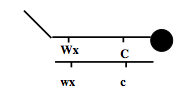
\includegraphics[width=.4\linewidth]{./img/01_cromosomiMais.png}
  \caption{Prima del crossing-over}
  \label{fig:sub1}
\end{subfigure}%
\begin{subfigure}{.5\textwidth}
  \centering
  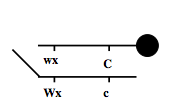
\includegraphics[width=.4\linewidth]{./img/02_crossingoverMais.png}
  \caption{Dopo il crossing-over}
  \label{fig:sub2}
\end{subfigure}
\caption{Cromosomi omologhi di mais presentanti marcatori genetici e citogenetici}
\label{fig:test}
\end{figure}

In seguito al crossing-over vi sarà la ricombinazione e il conseguente ottenimento di una progenie ricombinante. I ricombinanti, dal punto di vista fenotipico, avranno delle cariossidi:

\begin{itemize}
\item wx – C;
\item Wx –c.
\end{itemize}

Analizzando il cariotipo delle cariossidi ricombinanti sarà possibile osservare che i cromosomi hanno effettuato la ricombinazione poiché tra i due è avvenuto uno scambio fisico dei segmenti cromosomici; essi risulteranno infatti morfologicamente distinguibili.\\
L’esperimento appena spiegato rappresenta quindi una prova diretta che i geni si trovino sui cromosomi.

Un esperimento analogo venne effettuato nel 1931 da Stern, utilizzando il cromosoma X di Drosophila. I marcatori presi in considerazione furono:
\begin{itemize}
\item \textbf{carnetion (car)}, indicante il colore dell’occhio;
\item \textbf{bar (b)}, indicante la forma dell’occhio. 
\end{itemize}

In Drosophila l’allele dominante è indicato con il simbolo ``+'', mentre il recessivo con la sigla del gene coinvolto.
I cromosomi parentali presenteranno cromosomi X diversi: uno formato da due frammenti e l’altro con un prolungamento della regione centromerica. 
Anche in questo caso, come per il mais, l’individuo sarà un eterozigote strutturale ed eterozigote per carnetion e bar.

\begin{figure}[h]
\centering
\begin{subfigure}{.5\textwidth}
  \centering
  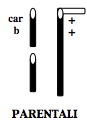
\includegraphics[width=.3\linewidth]{./img/03_cromosomiDrosophila.png}
  \caption{Prima del crossing-over}
  \label{fig:sub1}
\end{subfigure}%
\begin{subfigure}{.5\textwidth}
  \centering
  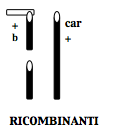
\includegraphics[width=.4\linewidth]{./img/04_crossingoverDrosophila.png}
  \caption{Dopo il crossing-over}
  \label{fig:sub2}
\end{subfigure}
\caption{Cromosomi omologhi di Drosophila presentanti marcatori genetici e citogenetici}
\label{fig:test}
\end{figure}

In seguito alla ricombinazione si otterrà un tipo ricombinante b/+ o car/+, ma anche cromosomi ricombinanti.

Questo esperimento dimostra, ancora una volta, che i cromosomi rappresentano la sede dei geni.


\subsection{Immagini}

\begin{figure}[h]
\centering
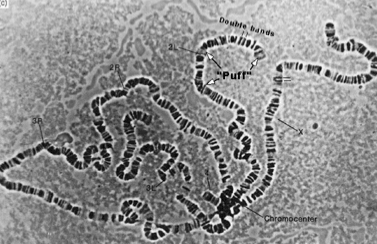
\includegraphics[scale=0.40]{img/04_cromo.png}
\caption{Immagine in contrasto di fase di cromosomi politenici non colorati}
\label{}
\end{figure}

\begin{figure}[h!]
\centering
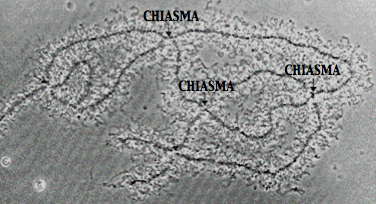
\includegraphics[scale=0.40]{img/05_cromospazzola.png}
\caption{Cromosomi a spazzola o lamp-brush, si tratta di cromosomi giganti che hanno avuto una particolare importanza per lo studio della sintesi dell’RNA. Sono presenti in tutti gli organismi, ma sono ben distinguibili in Xenopus laevis}
\label{}
\end{figure}

\begin{figure}[h!]
\centering
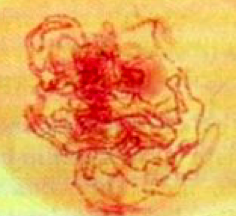
\includegraphics[scale=0.50]{img/06_cromopachitenespazzola.png}
\caption{Cromosomi in pachitene, una delle fasi della prima profase meiotica. Anche in questo caso si tratta di cromosomi a spazzola, ma non altrettanto ben studiabili come quelli giganti di Xenopus}
\label{}
\end{figure}

\begin{figure}[h!]
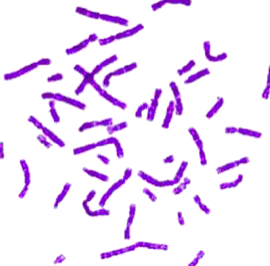
\includegraphics[scale=0.50]{img/07_cromoumani.png}
\centering
\caption{Colorazione standard di cromosomi umani in metafase. I cromosomi sono colorati in modo uniforme con un colorante affine al DNA}
\label{}
\end{figure}

\begin{figure}[h!]
\centering
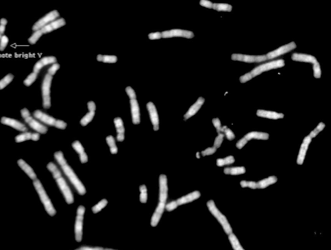
\includegraphics[scale=0.50]{img/08_cromobandeggi.png}
\caption{Particolarmente importante fu l’introduzione delle tecniche di bandeggio. Questa immagine mostra uno dei primi bandeggi storicamente sviluppati all’inizio degli anni `70 nel quale è possibile osservare delle regioni trasversali più o meno intensamente fluorescenti}
\label{}
\end{figure}

\begin{figure}[h!]
\centering
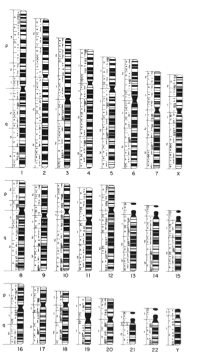
\includegraphics[scale=1.0]{img/09_cariotipo.png}
\caption{Successivamente vennero sviluppati altri bandeggi, questi furono fondamentali per l’identificazione dei cromosomi e per lo studio delle patologie cromosomiche. 
Per il riconoscimento dei cromosomi si utilizzano degli ideogrammi, questi rappresentano uno schema e vengono usati come riferimento per la descrizione di un cariotipo. Nell’ideogramma ogni banda rappresenta una rata(?) in modo tale che quando viene descritto un ri-arrangiamento cromosomico sarà possibile definire su che cromosoma ci si trova (braccio corto o lungo) e quali bande coinvolgano i punti di rottura.
Viene inoltre utilizzata una classificazione internazionale in modo che la descrizione del cariotipo sia universalmente comprensibile.
L’immagine a fianco mostra l’ideogramma di una metafase in cui la risoluzione è di sole 450 bande e una in cui invece la risoluzione è di 1700 bande. Non si tratta di una risoluzione elevata se si pensa che con i massimi livelli si arriva a distinguere fino a 3000 bande su un cariotipo umano. Sarà quindi possibile descrivere anche dei dettagli di riarrangiamenti molto piccoli, ciò risulterà essere fondamentale in molte patologie, ma soprattutto nel cancro}
\label{}
\end{figure}

\begin{figure}[h!]
\centering
\begin{subfigure}{.5\textwidth}
  \centering
  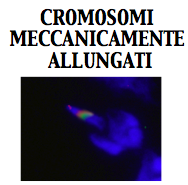
\includegraphics[width=.7\linewidth]{img/10_cromoallungati.png}
  \caption{}
  \label{fig:sub1}
\end{subfigure}%
\begin{subfigure}{.5\textwidth}
  \centering
  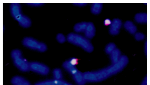
\includegraphics[width=1.1\linewidth]{img/11_cromoallungati.png}
  \caption{}
  \label{fig:sub2}
\end{subfigure}
\caption{Nell’immagine è possibile osservare l’utilizzo di una tecnica molecolare che permette di identificare determinate regioni cromosomiche con delle sonde molecolari. E’ possibile osservare una sonda marcata in verde e una in giallo. 
È possibile aumentare la risoluzione, potendo così cogliere più dettagli, utilizzando una tecnica che permette di stirare come degli elastici i cromosomi, nota come tecnica dei cromosomi meccanicamente allungati. }
\label{fig:test}
\end{figure}

\begin{figure}[h!]
\centering
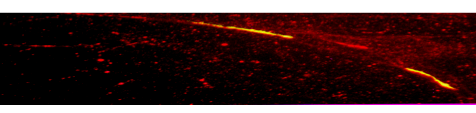
\includegraphics[scale=0.80]{img/12_cromatinapettinata.png}
\caption{Vi sono poi delle tecniche che permettono di pettinare la cromatina sui vetrini, di stabilire come siano disposte le diverse sequenze, quali siano i rapporti relativi (cosa si trova a destra piuttosto che a sinistra) e anche la distanza tra le diverse sequenze}
\label{}
\end{figure}

\begin{figure}[h!]
\centering
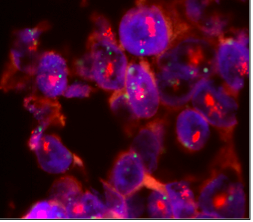
\includegraphics[scale=0.70]{img/13_celltumorali.png}
\caption{Nell’immagine a fianco è possibile osservare un caso di identificazione, con approcci molecolari, di regioni amplificate nel cancro alla mammella. Ciò risulta essere fondamentale perché permette di capire quale sia il grado di progressione della patologia.
Il gene marcato in rosso risulta essere molto amplificato nelle cellule tumorali, rappresenterà quindi una fase avanzata della malattia. 
Questo tipo di indagine è fondamentale perché permette di capire il livello di gravità e progressione del tumore, ma anche di fare la stessa analisi al termine di un trattamento terapeutico per osservare se vi sia stata una regressione del tumore. }
\label{}
\end{figure}


\begin{figure}[h!]
\centering
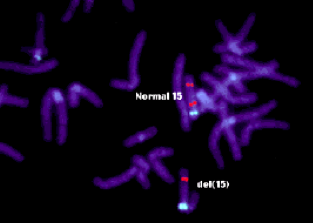
\includegraphics[scale=0.60]{img/14_microdelezioni.png}
\caption{La citogenetica molecolare può essere utilizzata anche per identificare delle micro-delezioni che non sarebbero visibili neppure con i  bandeggi ad alta risoluzione. L’immagine mostrante questa tecnica fa riferimento alla sindrome di prader-willi, molto studiata a causa del fenomeno dell’imprinting genomico}
\label{}
\end{figure}

\begin{figure}[h!]
\centering
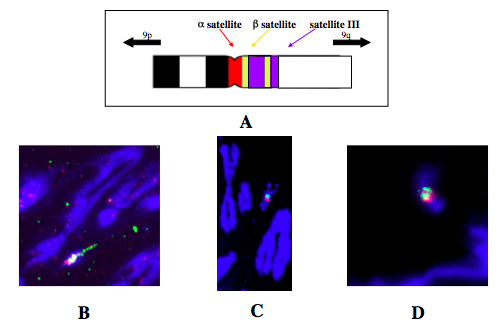
\includegraphics[scale=0.50]{img/15_cromoartificiale.png}
\caption{L’immagine a fianco mostra il lavoro che è stato fatto nel laboratorio della docente, in cui è stata fatta una mappa ad alta risoluzione della regione centromerica di un cromosoma umano, osservando quale fosse la sequenza e l’organizzazione dei diversi satelliti centromerici in una condizione normale e dopo aver costruito, attraverso delezioni successive, un cromosoma artificiale. 
Con i diversi gradi di risoluzione è possibile osservare i rapporti tra le diverse sequenze e la presenza/assenza di alcune delle stesse, marcate in fluorescenza con colori differenti}
\label{}
\end{figure}


\begin{figure}[h!]
\centering
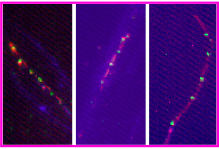
\includegraphics[scale=1.00]{img/16.png}
\caption{Nell’immagine sono stati analizzati i cromosomi allungati meccanicamente. In questo caso ciò che è interessante da osservare è non solo la struttura del centromero, ma anche la presenza di sequenze telomeriche. In questo caso era stato clonato, all’interno di un sito di clonaggio di un cromosoma artificiale, un gene marcatore (in verde nella figura) che risulta essere presente in 5 copie integrate}
\label{}
\end{figure}

\begin{figure}[h!]
\centering
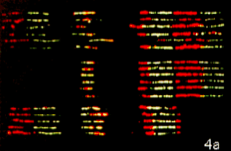
\includegraphics[scale=1.00]{img/17.png}
\caption{L’immagine a fianco mostra l’analisi di mutazioni del gene codificante per la distrofina su fibra di cromatina estesa.
Si tratta di un’immagine di un lavoro derivante dalla letteratura che prende in considerazione la distrofia di Duchenne. Il gene della distrofina è il gene più grande fino ad oggi clonato del genoma umano che quando mutato determina, appunto, la sindrome di Duchenne, una malattia invalidante abbastanza frequente. Risulterà quindi importante caratterizzare le diverse mutazioni sia per la diagnosi che per tentare degli approcci terapeutici mediante terapia genica.
In questo caso è stata costruita la mappa delle delezioni del gene della distrofina in diversi pazienti attraverso tecniche di citogenetica molecolare ad alta risoluzione grazie alle quali è possibile identificare i segmenti mancanti nelle differenti situazioni; ciò risulterà essere importante perché permetterà poi di vedere quali siano le delezioni più frequenti e, quindi, effettuare una diagnostica mirata}
\label{}
\end{figure}

\begin{figure}[h!]
\centering
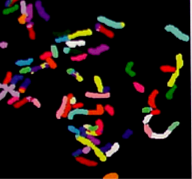
\includegraphics[scale=0.80]{img/18.png}
\caption{L’immagine a fianco mostra l’utilizzo di tecniche molecolari a più colori che permettono di colorare i cromosomi in modi differenti e di effettuare delle analisi in cui i ri-arrangiamenti cromosomici, anche molto complessi, potranno essere identificati grazie proprio allo scambio di colori tra i cromosomi. 
Se ogni cromosoma possiede un colore proprio, sarà possibile trovare un cromosoma arlecchino formato da diversi tasselli di provenienza nota. 
Quando si ha a che fare con ri-arrangiamenti che possono avere anche 10-11 punti di rottura, è chiaro che un bandeggio non permette di capire quali siano i punti di rottura dei cromosomi coinvolti; queste nuove tecniche, note come sky fish o spectral karyotyping, permetteranno invece di vedere anche ri-arrangiamenti molto complessi e di indirizzare l’analisi e la ricerca degli esatti punti di rottura}
\label{}
\end{figure}

\begin{figure}[h!]
\centering
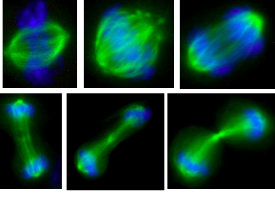
\includegraphics[scale=0.70]{img/19.png}
\caption{A fianco sono mostrate delle immagini di immunofluorescenza del fuso mitotico e dei cromosomi che permettono di osservare se vi siano delle anomalie di segregazione dei cromosomi rilevabili attraverso modificazioni della struttura del fuso mitotico. 
Generalmente si tratta di anomalie riguardanti il centromero}
\label{}
\end{figure}

\begin{figure}[h!]
\centering
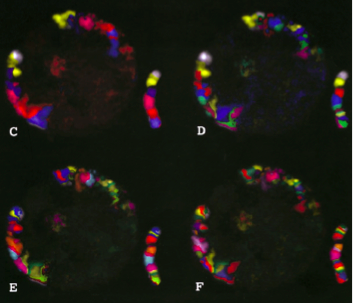
\includegraphics[scale=0.60]{img/20.png}
\caption{Ad oggi vi sono delle tecniche, risultanti fondamentali, che permettono di studiare i cromosomi nel nucleo interfasico. Nell’immagine è infatti possibile osservare dei nuclei
interfasici dove ciascuna banda di una particolare coppia di cromosomi è colorata in modo differente, sarà così possibile osservare l’organizzazione nel nucleo interfasico dei diversi distretti cromosomici. Ciò risulta essere molto importante perché è stato scoperto che la distribuzione tridimensionale dei vari domini cromosomici nel nucleo interfasico è direttamente correlata alla funzione degli stessi e che modificazioni della distribuzione si hanno nel corso del ciclo cellulare e possono anche essere indice di particolari perturbazioni dello stesso o di determinati pathway metabolici}
\label{}
\end{figure}

\begin{figure}[ht!]
\centering
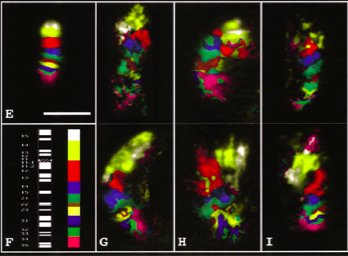
\includegraphics[scale=0.70]{img/21.png}
\caption{Queste tecniche permettono di fare un bandeggio cromosomico a più colori e vedere, nel nucleo interfasico, come sono organizzati i diversi distretti cromosomici. 
Questi approcci prevedono inoltre delle analisi tridimensionali del nucleo interfasico. È possibile arrivare a misurazioni e a simulazioni tridimensionali della disposizione di tutti i domini, queste risulteranno essere particolarmente importanti per fare delle deduzioni sull’importanza della posizione di particolari regioni cromosomiche nel nucleo interfasico e del loro significato funzionale}
\label{}
\end{figure}

\clearpage
La citogenetica del futuro è, fondamentalmente, la citogenomica; quest’ultima non vuole sostituire la citogenetica morfologica al microscopio, si tratta infatti di una disciplina che prevede l’utilizzo dei micro-array. Si parla quindi di citogenomica poiché rappresenterà un tipo di citogenetica fatta mediante approcci di genomica. 

\chapter{L'organizzazione del DNA}

A differenze dei procarioti, negli organismi eucarioti il grosso della regolazione dell'espressione genica avviene grazie a modificazioni del grado di condensazione del DNA, per questa ragione è molto importante conoscerne l'organizzazione.

In questo corso verranno approfonditi quei meccanismi che, modificando il grado di condensazione della cromatina (non è corretto parlare solo di DNA in quanto questo è complessato con le proteine istoniche), modulano la funzione delle cellule sia durante il ciclo cellulare che durante lo sviluppo e il differenziamento.
Il primissimo livello di regolazione dell’espressione genica negli eucarioti è dunque di carattere epigenetico. È evidente che siano importanti le sequenze regolatrici (promotori, enhancers, silencers, ecc), tuttavia l’attività di queste sequenze è modulata dalla loro accessibilità e quindi dal grado di condensazione della cromatina.

Prendiamo come punto di riferimento il genoma umano: nell’uomo la quantità totale in peso/massa di DNA è enorme, \emph{300 milioni bp} in aploidia. Se facciamo il conto, moltiplicando i 300 milioni per l’ingombro di ogni singola base, arriviamo ad una quantità di DNA pari a \textbf{1,80 metri} di lunghezza. Abbiamo dunque un'enorme sproporzione tra la dimensione del DNA e la dimensione del comparto in cui esso deve essere contenuto, e cioè il nucleo, il cui ordine di gradezza è quello dei micrometri. 

Si pone dunque il problema di come riuscire a condensarlo affinchè possa stare al suo interno: il DNA è una molecola molto sottile che potrebbe essere contenuta nel nucleo semplicemente comprimendola al suo interno ma, dal momento che circa ogni 24h il DNA di una cellula deve essere ripartito correttamente in due cellule figlie, è evidente che questo non può essere una matassa caotica ma deve essere rapidamente districabile. 
Il DNA raggiunge il suo massimo grado di condensazione durante la divisione cellulare (condensazione massina in metafase) e i cromosomi diventano dei ``gomitolini'' ben distinti con un livello di condensazione tale da renderli morfologicamente ben delineati e facilmente identificabili e classificabili al microscopio.

Il DNA è diviso in cromosomi, e negli essere umani la lunghezza totale di 1,80 metri è divisa in 23 coppie di cromosomi. Nell'organizzazione del DNA è poi molto importante che regioni che sono in qualche modo funzionalmente correlate ma linearmente molto distanti tra di loro, debbano potersi trovare vicine in certi momenti del ciclo cellulare, dello sviluppo e/o del differenziamento, in modo da poter essere espresse o replicate (replicazione e espressione sono fenomeni concertati) in maniera coordinata. È dunque fondamentale l'esistenza di meccanismi che permettano a tratti di DNA che, se consideriamo la molecola lineare, sarebbero molto distanti tra di loro di trovarsi in condizione di poter rispondere agli stessi segnali regolativi: si tratta fondamentalmente di meccanismi epigenetici di regolazione dell’espressione genica.

Qual è la soluzione ai problemi che abbiamo esposto? Com'è possibile che tutto il DNA entri nel nucleo?
Per risolvere questo problema il DNA viene condensato in modo ordinato, secondo una sequenza gerarchica di superavvolgimenti.
In generale il modello che viene seguito è il \textbf{modello a spirale}, un modello molto frequente in biologia e in tutto il mondo naturale in quanto, dal punto di vista fisico, è un modello energeticamente economico, ovvero è il modello che permette di ottenere forme ordinate con il minor dispendio di energia.


Vediamo alcuni rapporti tra dimensione del genoma e dimensione del comparto in cui questo è contenuto:
\begin{itemize}
\item Il \textbf{virus del mosaico del tabacco} è un virus filamentoso la cui dimensione è di 0.008 x 0.3  micron. Ha un genoma la cui lunghezza è di 6.4 Kb che corrispondono a 2 m. In questo caso non c’è una sproporzione così esagerata tra dimensioni del comparto/cellula/virus e dimensioni del genoma.
\item Il \textbf{Fago T4}, una cellula icosaedrica, ha una dimensione di 0.065 x 0.10 microm. Qui la sproporzione è già più evidente perché il genoma è di 170 Kb, per una lunghezza di 55 m.
\item \textbf{E. coli} è un batterio cilindrico tra i più conosciuti in quanto ampiamente utilizzato come organismo modello, della dimensione di 1.7 x 0.65 m. Il suo genoma è costituito da 4.2 x 103 Kb e ha una lunghezza di 1.3 mm (non più m).
\item Il \textbf{genoma umano aploide} è di \textbf{3x10\(^9\) Kb}, un genoma diploide è di 6 x 10\(^9\) Kb pari ad 1.80 metri. Il DNA umano è poi suddiviso in 46 cromosomi, ognuno dei quali è costituito da una molecola di DNA di circa 8 cm (la dimensione dei cromosomi è variabile), mentre il nucleo somatico sferico ha una dimensione di 6 micron (i nuclei delle cellule uovo sono molto più grandi).
\end{itemize}

La sproporzione tra la dimensione del genoma e quella del comparto in cui deve essere contenuto è evidente in tutti gli organismi e in particolare negli eucarioti superiori.
Una cosa fondamentale è che la cromatina, nelle cellule eucariotiche, viene trascritta e replicata in interfase.

Dal punto di vista energetico invece la fase più dispendiosa per la cellula è quella della divisione vera e propria, quando tutto il macchinario cellulare è concentrato sulla ipercondensazione della cromatina, sulla costruzione del fuso mitotico, sulla costruzione del cinetocore e su tutti quei processi che permettono la corretta separazione dei cromosomi nelle cellule figlie. Quando la cellula si divide la cromatina è ipercondensata: non viene né trascritta né replicata, salvo rarissime eccezioni.
Tutta l’attività metabolica della cellula invece si svolge durante l’interfase, quando il DNA è sì condensato perché deve stare nel nucleo, ma il grado di condensazione della cromatina è tale da consentire la funzionalità e la regolazione dell’espressione genica. 


\section{La cromatina}
Quando ci si riferisce agli eucarioti non bisognerebbe mai parlare di DNA ma di cromatina, in quanto normalmente il DNA è complessato con le proteine istoniche e solo transitoriamente è ``nudo''.

Gli istoni sono le proteine più abbondanti nel nucleo di una cellula eucariotica (rapporto in massa tra DNA e istoni di 1 a 1).

La cromatina viene divisa in \emph{eucromatina} ed \emph{eterocromatina}. Questa divisione è basata su osservazioni di microscopia ottica e si riferisce alla colorabilità con coloranti basici di diverse regioni del nucleo interfasico, distinguiamo:
\begin{itemize}
\item \emph{regioni più intensamente colorabili} che sono quelle più condensate durante l’interfase e sono le \textbf{regioni eterocromatiche}; 
\item \emph{regioni meno colorabili}, che sono quelle meno condensate durante l'interfase e sono le \textbf{regioni eucromatiche}.
\end{itemize}

Queste sono in realtà delle grosse generalizzazioni perché si basano soltanto su analisi morfologiche al microscopio ottico. In realtà, le regioni eucromatiche, come anche quelle eterocromatiche, contengono al loro interno rispettivamente regioni eterocromatiche e regioni eucromatiche: si tratta quindi di sub-regioni.

A sua volta l’eterocromatina si divide in:
\begin{itemize}
\item \textbf{eterocromatina costitutiva}. Questa è un'eterocromatina di tipo costituzionale, sempre presente a prescindere dalle fasi dello sviluppo, del differenziamento e del ciclo cellulare in cui una cellula di una certa specie si trova. Rappresenta una \emph{caratteristica intrinseca di una certa regione del genoma}. Questo tipo di eterocromatina è sempre presente in una determinata regione del genoma in tutte le cellule di tutti gli organismi della stessa specie.\\
In realtà ad oggi questo concetto è stato ampiamente messo in discussione.
Esempio eclatante: quando parliamo di eterocromatina costitutiva tipicamente ci vengono in mente le regioni centromeriche di tutti i cromosomi, ma oggi sappiamo che la regione centromerica non è completamente eterocromatica anzi, ad essere eterocromatica è la regione \emph{pericentromerica} che forma una sorta di barriera e che contiene al suo interno il core funzionale centromerico trascrizionalmente competente.
\item \textbf{eterocromatina facoltativa}. Questa eterocromatina è presente soltanto in certe condizioni, può variare, e quindi non caratterizza la struttura di una certa regione cromosomica. 
Questo tipo di eterocromatina può riguardare certe regioni del genoma solo in alcune cellule di alcuni organismi della stessa specie oppure può riguardare soltanto uno degli omologhi.\\
L’esempio meglio studiato di eterocromatina facoltativa è il cromosoma X inattivo nelle cellule somatiche delle femmine di mammifero (\textbf{N.B.:} l'inattivazione dell'X non riguarda solo l’uomo ma tutti i mammiferi e, più in generale, tutti gli organismi con eteromorfismo dei cromosomi sessuali).
Questo è l’esempio meglio studiato di eterocromatina facoltativa, ma in natura ce ne sono molti altri (per esempio in alcuni insetti vengono inattivati tutti i cromosomi di origine paterna nelle cellule somatiche dei maschi, e questo è un meccanismo di determinazione del sesso).
\end{itemize}

\begin{figure}[h!]
\centering
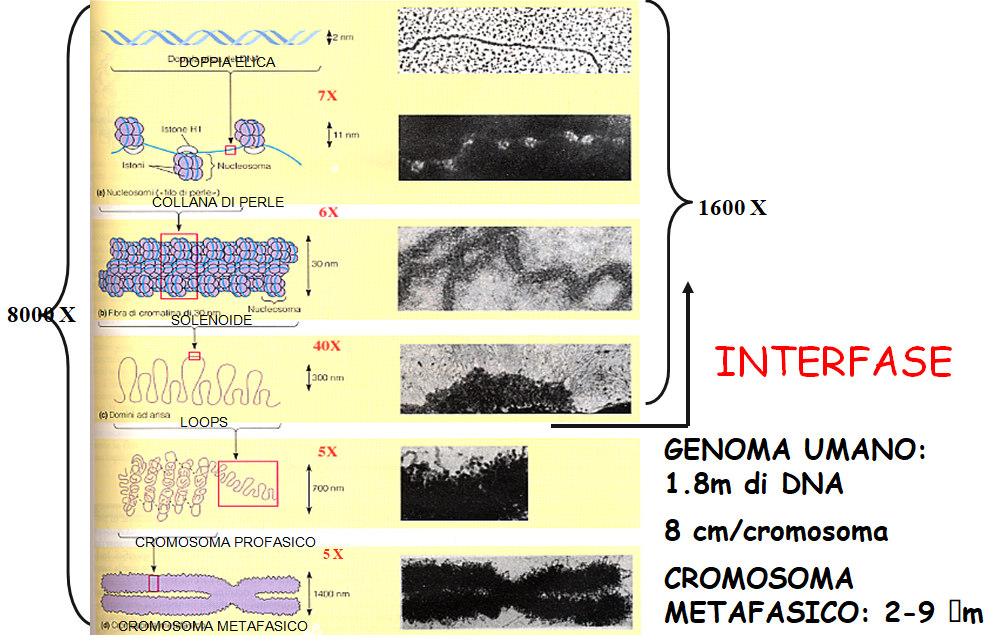
\includegraphics[scale=0.70]{img/22_cromatina.png}
\caption{Diversi livelli di condensazione del DNA. Possiamo vedere sia una rappresentazione schematica che l’immagine al microscopio elettronico. Inoltre nell’immagine si vede anche la dimensione, lo spessore, della fibra a cui ci riferiamo: il confronto di spessore delle fibre con ordine sempre superiore di superavvolgimento ci dà un’idea del grado di condensazione.}
\label{livelli_condensazione}
\end{figure}

Il ciclo di condensazione del DNA è rappresentato nell’immagine \ref{livelli_condensazione}, dove abbiamo una divisione molto netta tra ciò che riguarda l’interfase e ciò che riguarda invece le fasi successive all'interfase che portano alla divisione cellulare. La parte dell’interfase è quella che ci interessa di più perché è la fase in cui la cromatina funzionale è sì superavvolta ma in modo tale da poter comunque permettere la regolazione dell’espressione genica.\\
A partire dalla \emph{doppia elica} di DNA che ha un diametro di \textbf{20 \si{\angstrom}} (pari a 2 nm), passiamo alla struttura di ordine superiore che è la \emph{collana di perle} che si vede molto bene al microscopio elettronico e che ha un superavvolgimento di 7 volte per una dimensione di \textbf{11 nm}. Un’ulteriore condensazione di 6 volte porta dalla collana di perle alla \emph{struttura a solenoide} che ha un diametro di \textbf{30 nm}; si arriva poi alla \emph{struttura ad anse} che prevede un superavvolgimento di altre 40 volte per una dimensione di \textbf{300 nm} e una superavvolgimento totale di 1.600 volte per quanto riguarda la condensazione di DNA in interfase.\\
Le fasi successive seguono di nuovo un modello ad elica: abbiamo un superavvolgiemento di 5x5 volte che porta al cromosoma profasico e poi al cromosoma metafasico che raggiunge il massimo della condensazione.

Il modello seguito per il superavvolgimento è sempre quello a spirale:
\begin{itemize}
\item La doppia elica è un modello a spirale;
\item La collana di perle è un modello a spirale perché il DNA su ogni nucleosoma si superavvolge con due spire;
\item Il modello a solenoide è un modello a spirale perché in ogni giro del solenoide ci sono 6 perle della collana di perle;
\item Il \textbf{modello a loop} invece \underline{non è} un modello a spirale ma è un \emph{modello variabile}: a variare è sia la dimensione dei loop che il loro grado di affastellamento, di condensazione. È questa la parte più importante su cui ci soffermeremo perché ha un significato regolativo fondamentale.
\end{itemize}

Il processo di condensazione del DNA porta dunque da una fibra di 1,8 m a cromosomi singoli in cui mediamente il DNA è lungo 8 cm per cromosoma (in realtà, al microscopio, i cromosomi metafasici umani, ipercondensati, hanno una dimensione che varia da 2 a 9 micron circa).

Parliamo ora della struttura della cromatina: con questo termine ci si riferisce infatti alla fibra di DNA complessata con le proteine istoniche (basiche) con un rapporto in massa di 1:1.
Gli istoni sono in assoluto le proteine più abbondanti nel nucleo di una cellula eucariote.
La fibra elementare, e cioè la collana di perle, ha un diametro di circa 10-11 nm e deve il suo nome alla ripetizione assolutamente regolare di strutture globulari chiamate \textbf{nucleosomi}. Ogni nucleosoma/perla è poi legato all'altro da un segmento di DNA chiamato \textbf{DNA linker}.

I nucleosomi sono costituiti da un core proteico, che forma la struttura glomerulare, formato da un ottamero di istoni. Gli istoni sono 5: \textbf{H1}, \textbf{H2a}, \textbf{H2b}, \textbf{H3} e \textbf{H4}.
A formare il nucleosoma partecipano solo gli istoni\emph{ H2A, H2B, H3 e H4} con due subunità per tipo.\\
In questo momento l’istone H1 non partecipa ancora alla condensazione.

Su ogni nucleosoma si superavvolgono \textbf{2 spire di DNA} per un totale di circa \textbf{140-150 pb}.\\
Le perle poi sono unite tra loro da un ``filo'', che è il \textbf{DNA linker}, lungo circa \textbf{50 pb}.

\begin{wrapfigure}{r}{0.3\textwidth}
    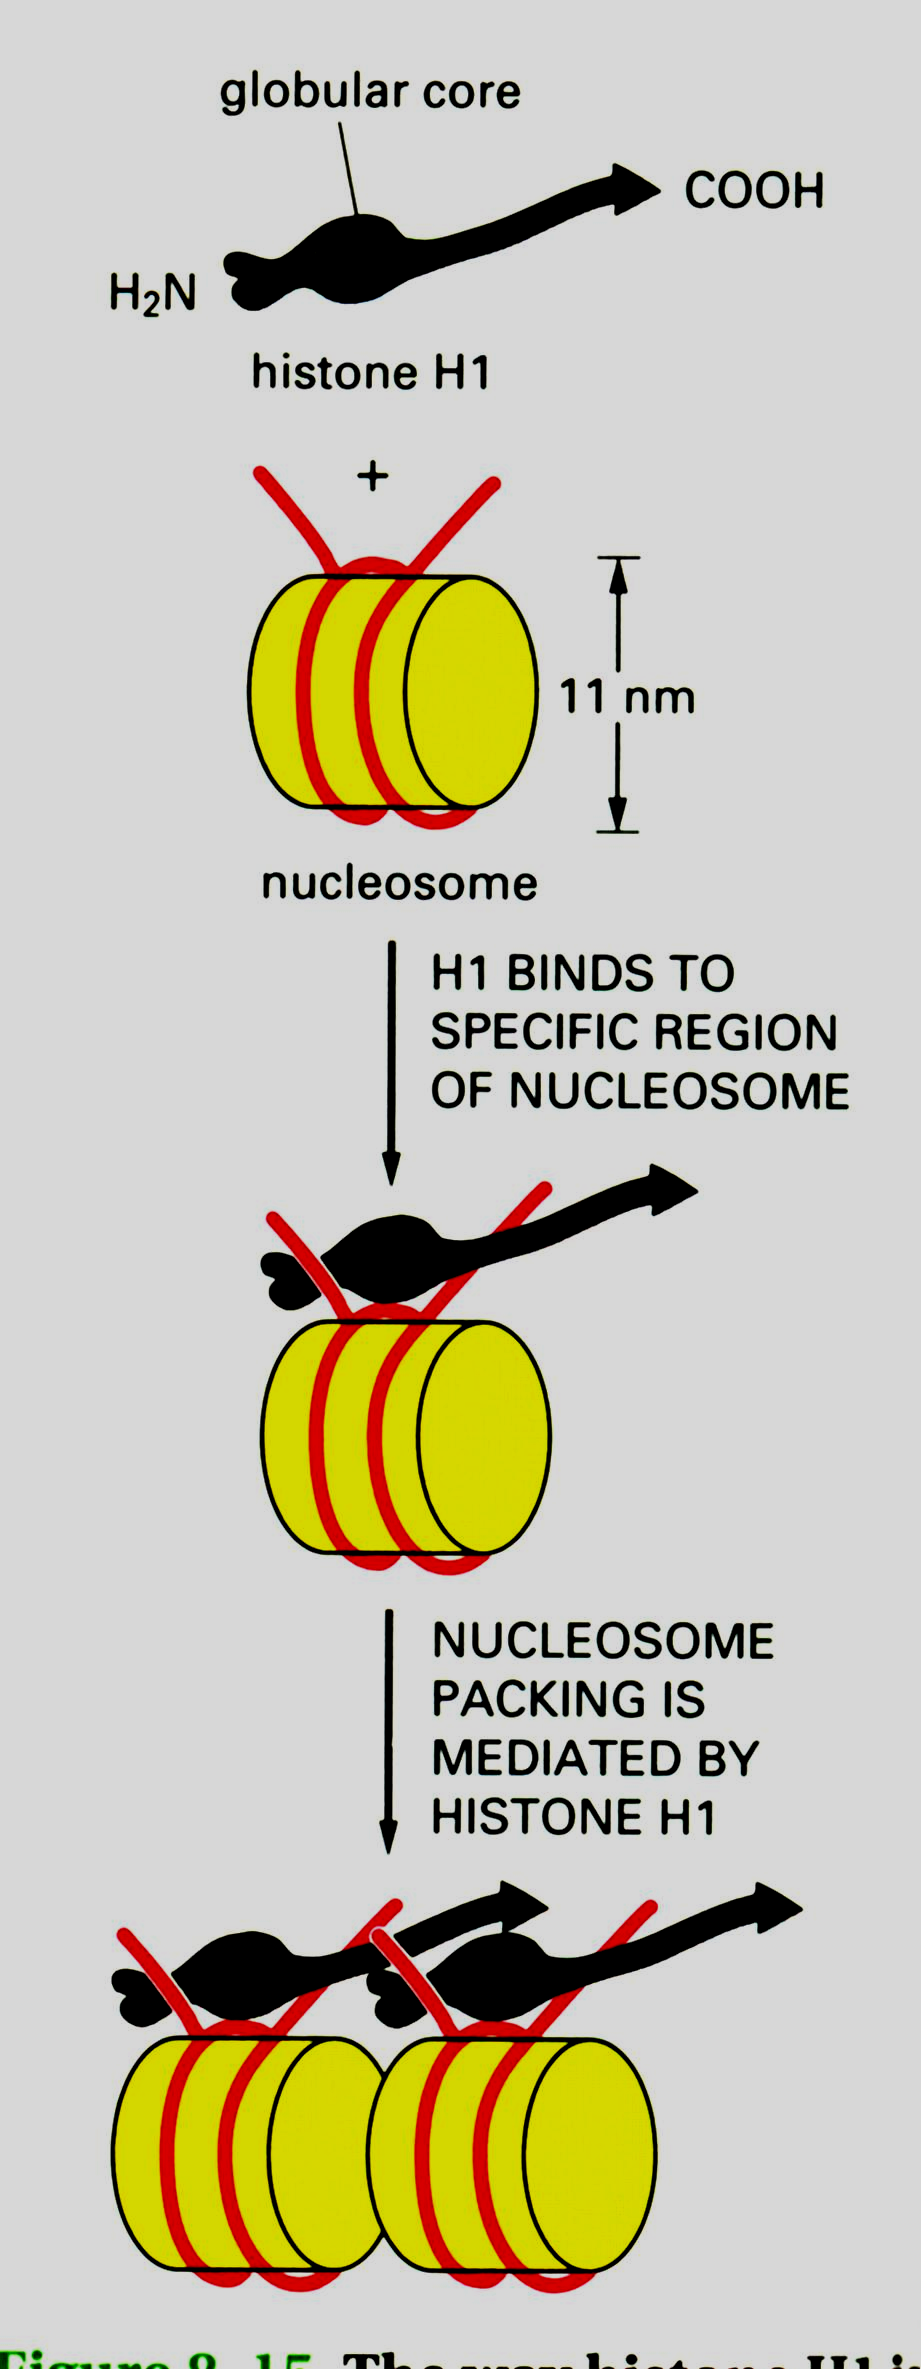
\includegraphics[width=0.27\textwidth]{img/23_histoneH1.png}
  \caption{Istone H1}
\end{wrapfigure}

L’\textbf{istone H1} invece si trova all’esterno rispetto all’ottamero e il suo compito è quello di collegare tra loro nucleosomi adiacenti determinando il superavvolgimento di ordine superiore, quello che porta alla formazione del \emph{solenoide}: in ciascun giro del solenoide si trovano \textbf{6 nucleosomi}, per portare alla struttura della fibra di 30 nm.

L’istone H1 nell’immagine di fianco è rappresentato come una specie di girino, con una testa (estremità C-terminale), una coda (estremità N-terminale) e una pancia. 
La pancia fornma la regione che interagisce con il DNA che si trova superavvolto sul nucleosoma, mentre la testa e la coda servono per i legami proteina-proteina che permettono la contrazione della fibra, in quanto l’istone H1 è legato all’esterno del nucleosoma attraverso un'interazione DNA-proteina.

Fino a questo livello di superavvolgimento c’è un motivo monotono ricorrente del modello a spirale che è più o meno uguale in tutti gli organismi e che segue questo ordine gerarchico. È un modello difficilmente modulabile fermo restando che, quando il DNA si deve replicare e deve essere trascritto, le proteine istoniche si devono staccare molto rapidamente per liberarlo.
Non è un caso che non abbiamo mai parlato di legami covalenti: queste sono tutte interazioni di tipo elettrostatico, fondamentalmente ponti H, proprio perché richiedono una bassa energia, sono facilmente reversibili e facilmente ricostruibili nel momento in cui si è compiuto il processo di replicazione e trascrizione.

\textbf{[DOMANDA:} il modello a zig-zag per quanto riguarda la fibra a 30nm non viene considerato? Il modello a zig-zag si ha quando il DNA linker ha una maggiore dimensione. Sono tutte variazioni sul tema: ci sono anche altri modelli più o meno validi e più o meno dimostrati, ma il modello più attendibile è quello a solenoide. Il modello a zig-zag si riferisce forse ad una sorta di ibrido tra il modello a solenoide e la struttura a loops.\textbf{]}

\subsection{La struttura a loops}

\begin{wrapfigure}{r}{0.3\textwidth}
    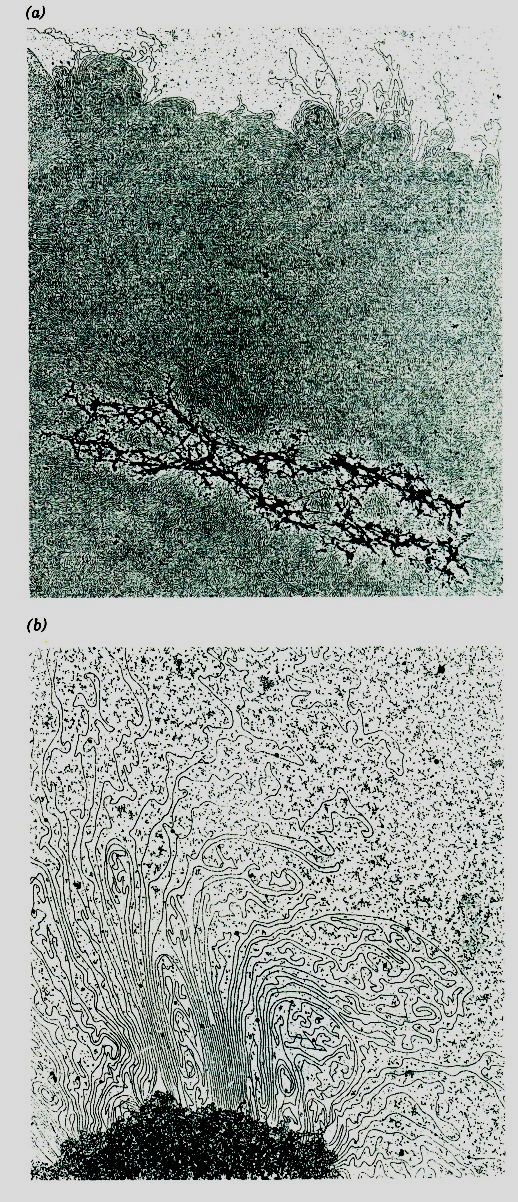
\includegraphics[width=0.30\textwidth]{img/25_backbone.png}
  \caption{Istone H1}
\end{wrapfigure}

È possibile trattare un cromosoma metafasico con una sostanza che permette di staccare gli istoni e che quindi permette la completa decondensazione (se tolgo gli istoni tutte le strutture di  ordine inferiore ovviamente si perdono). Osservando al microscopio elettronico il cromosoma metafasico trattato con questa sostanza vediamo che resta uno scheletro, chiamato \emph{``back bone''}, che rispecchia la morfologia del cromosoma metafasico. Tuttavia, a partire da questa sorta di colonna vertebrale che rimane, si vedono delle estensioni/estroflessioni che formano una sorta di alone intorno ad esso. Aumentando l’ingrandimento si può vedere come questo alone che si estroflette dal back bone sia costituito da fibre molto sottili che rappresentano delle anse continue: le anse si estroflettono a partire dallo scheletro per poi riattaccarvisi.\\
Queste analisi al microscopio elettronico sono la dimostrazione morfologica della struttura ad anse della cromatina, una struttura molto variabile e non sempre presente. Questa struttura, nonostante vari tra regioni diverse e a seconda della funzionalità, è effettivamente una struttura portante in metafase.
Quindi la cromatina interfasica ha una struttura ad anse.

Esistono delle evidenze della struttura ad anse: immagini in microscopia elettronica, esperimenti di sedimentazione, esperimenti di digestione con nucleasi. Tutti queste esperimenti hanno permesso di caratterizzare gli elementi di questa struttura.\\
Le anse sono delle \textbf{unità funzionali}: ci sono diverse prove sperimentali che dimostrano che le anse sono più o meno definibili come delle unità funzionali e cioè delle unità di trascrizione e di replicazione (eventi concertati). 
La struttura ad anse varia a seconda delle esigenze funzionali della regione cromosomica in un certo momento dello sviluppo e in un certo tipo cellulare. Ha un ruolo fondamentale nella regolazione dell’espressione genica e cioè nella trascrizione.

Regola generale, ma non sempre è così: tutto ciò che è attivamente trascritto è anche replicato all’inizio della fase S del ciclo cellulare, tutto ciò che è silenziato è invece replicato alla fine della fase S del ciclo cellulare.
Quello che è altamente condensato è poco trascritto ed ha replicazione tardiva. Quello che è poco condensato è attivamente trascritto ed ha replicazione precoce (durante la fase S iniziale). Questo avviene proprio perché trascrizione e replicazione sono processi metabolici interconnessi.

Lo scheletro proteico che è costituito dalla \textbf{topoisomerasi II}, la quale rappresenta la seconda proteina per abbondanza in massa nel nucleo delle cellule eucariotiche.

L’\emph{asse dell’ansa} è dunque il DNA complessato con gli istoni, mentre la \emph{base dell’ansa} è l’impalcatura che abbiamo visto bene nelle immagini di microscopia elettronica, chiamata \textbf{chromosome scaffold} (matrice del cromosoma) e costituita fondamentalmente dalla topoisomerasi II.

Che la base delle anse sia formata da delle topoisomerasi non è un caso, infatto queste sono proteine fondamentali durante la replicazione e la trascrizione perchè capaci di indurre tagli a singolo e a doppio filamento fondamentali per rilassare le tensioni torsionali che si vengono a creare quando il DNA si decondensa e quando la doppia elica si svolge. Se la doppia elica venisse semplicemente svolta ed aperta si sviluppere una tensione che potrebbe causare delle rotture casuali della molecola di DNA: affichè questo non avvenga ci sono le topoisomerasi che inducono dei tagli mirati a singola elica che vengono poi saldati e servono ad evitare che queste tensioni torsionali portino ad anomalie e ad errori nella replicazione e nella trascrizione.

Il fatto che la topoisomerasi II si trovi alla base delle anse ha un senso se è vero che le anse sono delle unità di trascrizione e di replicazione. La topoisomerasi ha dunque sia una funzione strutturale che enzimatica.
   
 Inoltre l'organizzazione a loops ha un significato molto importante perché ovviamente, se noi creiamo un’ansa anche molto grande, facciamo in modo che regioni fisicamente molto lontane sulla molecola lineare di DNA vengano a trovarsi invece molto vicine.\\
L’organizzazione a loops è dunque in grado anche di tenere fisicamente vicine regioni che devono essere trascritte o replicate nello stesso momento funzionale: queste regioni potranno trovarsi fisicamente vicine per rispondere agli stessi segnali regolatori.

A questo punto, siccome il loop ha un significato regolativo, è facile capire come la dimensione e il grado di condensazione dei loop varino in diversi stadi dello sviluppo e in diversi tessuti.

\begin{wrapfigure}{r}{0.62\textwidth}
    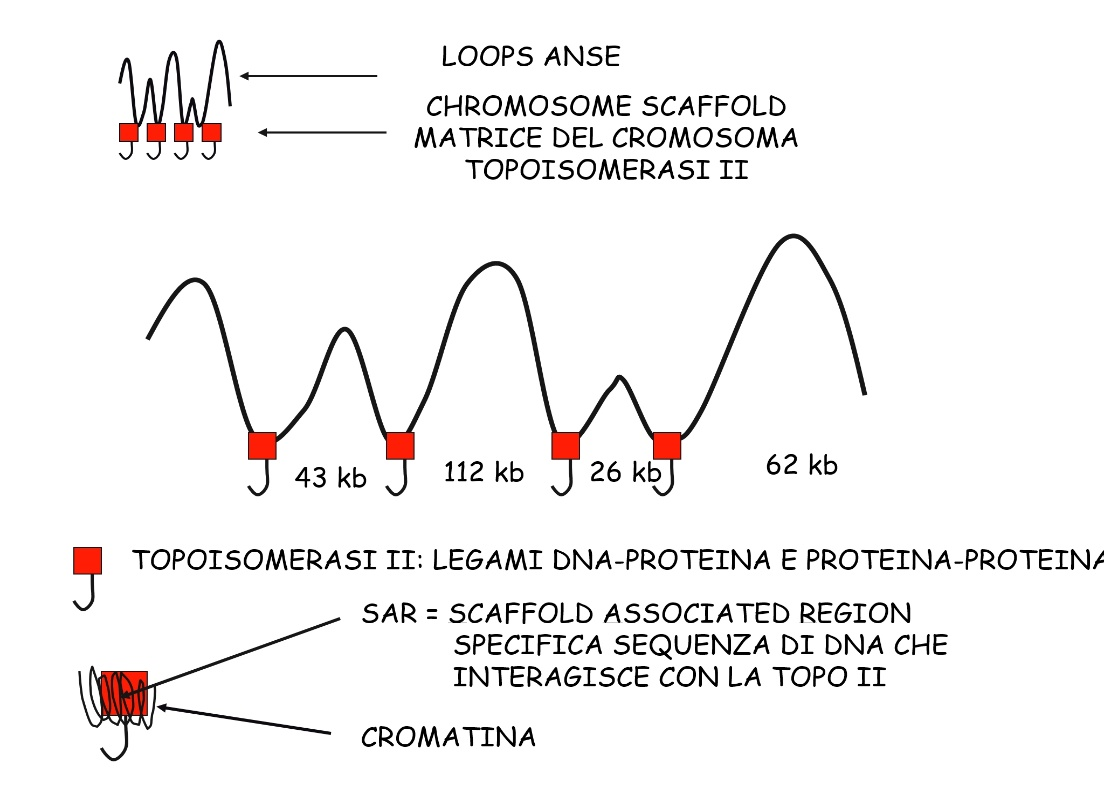
\includegraphics[width=0.60\textwidth]{img/26_anse.jpg}
  \caption{La topoisomerasi II e l'organizzazione ad anse}
\end{wrapfigure}

Il disegno a lato ci fa capire come la struttura a loops possa essere facilmente regolata e cioè come, grazie al legame della base delle anse con la topoisomerasi, siamo in grado di modulare la dimensione e il grado di affastellamento delle anse.\\
Nel disegno la topoisomerasi è rappresentata come una sorta di vagoncino con un occhiello: la parte rossa del vagoncino è quella su cui si trova la regione della topoisomerasi affine al DNA, e cioè la regione di interazione DNA-proteina: la parte rossa è legata alla base delle anse.\\
Il chromosome scaffold è dato dall’allineamento delle diverse molecole di topoisomerasi.

La topoisomerasi quindi è in grado di formare legami DNA-proteina che si trovano alla base dell’ansa, ma anche legami proteina-proteina che saranno i legami tra gli occhielli di molecole di topoisomerasi adiacenti. È evidente come questo permetta facilmente di modificare sia la dimensione che il grado di affastellamento dei loop.

Come faccio a modificare la dimensione dei loop?
Se ho due loop adiacenti, uno di 112 Kb e l’altro di 26 Kb, e tolgo la molecola di topoisomerasi compresa tra i due loop, succede che da due loop di quelle dimensioni ne ottengo uno più grande la cui dimensione sarà esattamente di 112 + 26 Kb.\\
Modulando semplicemente l’interazione DNA-proteina posso modulare la dimensione dei loop, mentre Per quanto riguarda il grado di condensazione è evidente che gli occhielli potranno interagire tra loro in modo lasso o stretto. La forza dell’interazione tra molecole di topoisomerasi adiacenti modulerà il grado di affastellamento dei loop e quindi il loro grado di condensazione.

Abbiamo detto che regione dove il DNA interagisce con la topoisomerasi si trova alla base dei loop, il DNA però può essere o meno legato alla topoisomerasi. Le regioni di DNA capaci di legarsi alle topoisomerasi si chiamano \textbf{SAR (Scaffold Associated Region)}.

Ciò che modula l'organizzazione ad anse è dunque l’interazione più o meno forte tra topoisomerasi (affastellamento), ma anche il legame o meno con la topoisomerasi (dimensione dei loop).

Ma se le regioni SAR sono sempre presenti, perché a volte legano la topoisomerasi  mentre altre volte no? È evidente che le stesse regioni SAR devono essere capaci o meno di legare la topoisomerasi, e questa capacità è determinata dalle modificazioni epigenetiche.\\
Epigenetica vuol dire che la stessa sequenza (o sequenze molto simili) può all’occorrenza trovarsi in una condizione tale da poter interagire con un fattore (in questo caso con una proteina) o meno.

La stessa molecola di topoisomerasi trova delle SAR disponibili o delle SAR incapaci grazie alla presenza di segnali chimici che rendeno le molecole di topoisomerasi in quella regione più affini rispetto a tutte le altre molecole di topoisomerasi. \emph{(la modificazione epigenetica è a livello delle SAR o della topoisomerasi??)}\\
Tutti questi sono segnali epigenetici perché la sequenza del DNA è sempre la stessa. Ad intervenire sono delle piccole molecole in grado di modificare localmente la struttura del DNA (in questo caso della SAR) rendendola aperta o chiusa, oppure di modificare la proteina rendendola più o meno affine alle altre proteine della sua stessa categoria.
Oggi sappiamo che queste piccole molecole sono RNA non tradotti. 

Questi cambiamenti epigentici sono essenziali se pensiamo che ogni loop è un'unità funzionale a sé stante. Nell'organizzazione del DNA possiamo fare una distinzione tra i geni housekeeping (geni che regola il metabolismo di base e che sono attivi in tutte le cellule) e geni tessuto-specifici.\\
I \textbf{geni housekeeping} regolano il metabolismo cellulare e sono trascritti in tutte le cellule ad un livello basale, mentre i geni tessuto-specifici vengono trascritti solo in certi tipi cellulari e sono trascritti a livelli molto più elevati.
A causa delle diverse esigenze di trascrizione l'organizzazione in loop di questi geni sarà diversa:
\begin{itemize}
\item i \textbf{geni housekeeping}, in generale, si trovano in loop piuttosto grandi e abbastanza condensati perché devono essere trascritti in maniera basale in tutte le cellule di tutti gli organismi. Nelle zone di \emph{eterocromatina costitutiva}, completamente inerti, troviamo loop molto grandi e molto molto condensati.
\item i \textbf{geni tessuto-specifici} invece si troveranno in loop piccoli e molto lassi (i.e. loop in cui si trova fondamentalmente un solo gene che viene continuamente trascritto). Quella stessa regione nella cellula di un altro tessuto sarà ipercondensata.
\end{itemize}

Se nei loop piccoli troviamo un solo gene o quasi e di conseguenza la trascrizione risulta molto rapida, i loop grandi conterranno unità trascrizionali che, venendo trascritte in sequenza, necessiteranno di tempi più lunghi.
Bisogna sempre ricordare che, durante la trascrizione e la replicazione, la doppia elica del DNA si deve aprire e i nucleosomi si devono staccare in maniera transiente per poi riattaccarsi subito dopo perché il DNA deve essere accessibile al complesso trascrizionale o al complesso replicativo. Affinchè questo avvenga, la cromatina deve essere in una conformazione adatta: si devono rapidamente staccare gli 8 istoni che formano il nucleosoma ma, appena completato il processo di trascrizione e di replicazione, gli istoni dell’ottamero si devono riassociare al DNA e tutto questo è modulato dalla struttura ad anse.
Le anse sono più o meno compatte e più o meno grandi nei diversi momenti funzionali e in diverse regioni cromosomiche: questo è variabile per le esigenze del differenziamento e dello sviluppo.


Cosa sono le modificazioni epigenetiche?\\
Sono cambiamenti della cromatina che regolano l’espressione genica a livello trascrizionale.
Tra i vari livelli di regolazione dell'espressione genica quello più economico è quello che interviene già a livello della trascrizione in quanto evita sprechi metabolici ed energetici.

Le modificazioni epigenetiche non alterano la sequenza del DNA ma la struttura tridimensionale della cromatina, hanno un ruolo chiave nei processi di regolazione dell’espressione genica negli eucarioti e rappresentano il sistema più usato per regolare l’espressione genica.
Le modificazioni epigenetiche non riguardano promotori, enhancers e silencers di per sé, ma piuttosto l’accessibilità di tali sequenze ai fattori con cui interagiscono. Le modificazioni epigenetiche fanno in modo che le sequenze regolatrici siano o meno capaci di interagire con i propri effettori.

Queste modificazioni consistono fondamentalmente in:
\begin{itemize}
\item metilazione del DNA;
\item metilazione ed acetilazione di specifici gruppi degli istoni che formano l’ottamero.
\end{itemize}

Una cosa fondamentale è che in ogni regione del genoma degli eucarioti superiori esiste un rapporto ben preciso tra grado di metilazione e grado di acetilazione e addirittura questo rapporto locale tra numero di acetili e numero di metili rappresenta una sorta di \textbf{codice istonico} che si sovrappone al codice genetico, proprio perché ha la capacità di modulare l’espressione genica locale. In qualche caso il codice istonico è stato decodificato: ci sono delle regioni del genoma in cui si è stabilito esattamente qual è il rapporto chiave tra metili e acetili e quindi il codice istonico per avere un certo livello di espressione genica. 

Le SAR sono state facilmente isolate e caratterizzate trattando il DNA con la stessa sostanza usata per ottenere il back bone proteico (litio 3’, 5 diiodiosalcilato, LIS), ovvero una molecola capace di rimuovere gli istoni. Rimuovendo gli istoni vi saranno delle regioni che risulteranno protette dal trattamento con enzimi di restrizione perché schermate dalla topoisomerasi. A questo putno posso rimuovere la topoisomerasi e caratterizzare i segmenti di DNA che erano stati protetti dalla digestione enzimatica: in questo modo sono state sequenziate le SAR.
Tutti questi esperimenti sono stati fatti fondamentalmente in Drosophila melanogaster.
Questo permette anche misurare la dimensione dei segmenti che si trovano tra due regioni protette dalla digestione enzimatica e quindi valutare la dimensione dei loops e dunque la distanza tra SAR adiacenti. In Drosophila la dimensione dei loops è molto variabile: da 4,5 a 115 Kb.


Tutte le SAR studiate contengono da 8 a 17 box ricorrenti: per \emph{``box''} si intende un blocco di sequenza: questi blocchi sono specifici e ricorrenti, molto simili tra loro in SAR diverse.\\
In tutte le SAR è presente un \emph{sito di legame per la topoisomerasi} costituito dalla sequenza \textbf{GNT(A/T)A(T/C)ATTNATNN(G/A)}. 
Vi sono poi altre due box ricorrenti (tra quelle trovate confrontando le diverse SAR della Drosophila melanogaster) dal significato regolativo: sono presenti o assenti a seconda che ci troviamo in una regione di geni housekeeping (che non devono essere regolati perché son trascritti in tutte le cellule di tutto l’organismo) o di geni tessuto-specifici (regolati). Abbiamo quindi una \textbf{T-box} che è un\emph{a\textbf{ sequenza ricca in T ed una \textbf{A-box} che è ricca in A}}. La T-box si trova a valle della A-box. La differenza tra geni housekeeping e geni  tessuto-specifici sta proprio in queste box regolative.
    • I geni housekeeping non sono regolati perchè sono trascritti a livello basale in tutti i tessuti e in tutti gli stadi del differenziamento: hanno delle SAR costitutive sempre legate alla topoisomerasi che mancano della A-box.
    • Le SAR regolate che si trovano adiacenti a geni tessuto-specifici trascritti ad alto livello soltanto in certi tessuti, presentano la A-box.
    • Una grossa differenza sta proprio in queste box regolative: fondamentale è la presenza o assenza della A-box rispettivamente nei geni tessuto-specifici (regolati) e nei geni costitutivi (housekeeping).

QUINDI:
    • Geni con alto livello di trascrizione (per esempio quelli tessuto-specifici) si troveranno in loop piccoli e lassi. Geni con basso livello di trascrizione si trovano in loop grandi e condensati.
    • Nei loop grandi ci sono più unità trascrizionali per cui la velocità di trascrizione ovviamente è inferiore. Nei loop piccoli invece c’è una sola unità trascrizionale e quindi la trascrizione è molto più rapida.
    • I loop hanno un significato funzionale: questo è dimostrato dal fatto che le SAR normalmente si trovano vicine ai promotori. Se noi facciamo un trattamento con enzimi di restrizione, considerando anche elementi regolativi a lunga distanza come gli enhancers, è molto facile che sullo stesso frammento di restrizione troviamo sia una SAR che un elemento regolativo a lunga distanza (enhancer).
    • La struttura a loop è tessuto specifica: se noi guardiamo la dimensione e il grado di affastellamento, questi sono variabili a seconda del tessuto che consideriamo.

































\end{document}